\setauthor{Elisa Kaltenberger}

Für einen Großteil der Bevölkerung stellt das Treppensteigen eine alltägliche Selbstverständlichkeit dar. 
Diese Selbstverständlichkeit erweist sich für einen geringen Anteil der Einwohner als nicht oder nur bedingt realisierbar. 
Menschen mit körperlichen Einschränkungen sehen sich im Alltag mit signifikanten Herausforderungen konfrontiert. 
Barrieren, die für andere kaum auffallen, können sich als unüberwindbare Hindernisse erweisen. Eine eingeschränkte 
Zugänglichkeit zu Infrastruktur und Dienstleistungen, wie beispielsweise ein nicht erreichbarer Geldautomat aufgrund eines
zu hohen Sichtschutzes oder das Fehlen eines Aufzugs oder einer Rampe, kann die Mobilität enrom einschränken und den 
Alltag erheblich erschweren. Der Fokus liegt dabei nicht ausschließlich auf Mobilität, sondern auch auf der gleichberechtigten 
Teilhabe am gesellschaftlichen Leben.

\section{Statistik}
In Österreich leben rund 1.9 Millionen Menschen im Alter zwischen 15 und 89 Jahren mit gesundheitlichen oder altersbedingten 
Einschränkungen. Dies entspricht etwa einem Viertel der Bevölkerung in dieser Altersgruppe. Die vorliegende Untersuchung 
Abb. \ref{fig:statistik-1}, 
befasst sich mit der Frage, inwiefern die genannte Personengruppe im Alltag von den Auswirkungen betroffen ist. Etwa 
7,6\% der Interviewten gaben an, dass sie sich bei typischen Aktivitäten wie Ankleiden, Einkaufen oder Haushaltsarbeiten durch
starke gesundheitliche Beeinträchtigungen erheblich eingeschränkt fühlen. Rund 17,5\% der Befragten berichteten zumindest eine
leichte Einschränkung.

Dies veranschaulicht, dass Einschränkungen im Alltag ein breites Spektrum umfassen - von leichten Beeinträchtigungen bis hin
zu Situationen, in denen selbst grundlegende Tätigkeiten ohne Hilfe kaum möglich sind. Eine Analyse der Gruppenzusammensetzung 
macht diese Tatsache besonders deutlich. Etwa 30,3\% der österreichischen Bevölkerung mit Behinderungen sind beeinträchtigt.

Die präsentierten Zahlen verdeutlichen, dass Barrierefreiheit und Unterstützungsangebote nicht als Randthema betrachtet
werden können, sondern für einen signifikanten Anteil der Einwohnerschaft von großer Bedeutung sind. Dabei geht es 
nicht nur um Mobilität oder medizinische Versorgung, sondern um die Möglichkeit, das eigene Leben selbstbestimmt zu gestalten 
und gleichberechtigt an der Gesellschaft teilzuhaben. In Anbetracht des demografischen Wandels wird die Relevanz 
barrierefreier Strukturen und inklusiver Maßnahmen in den kommenden Jahren deutlich ansteigen.

\begin{figure}
    \centering
    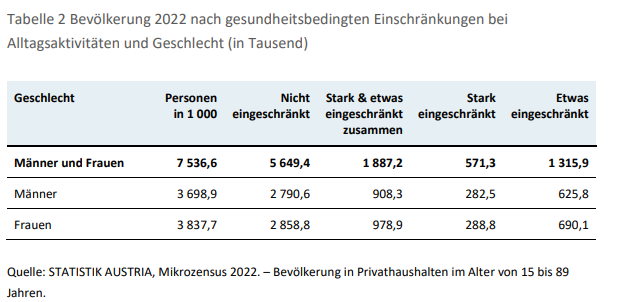
\includegraphics[scale=1]{pics/Statistik-Einschraekungen.png}
    \caption{Statistik Einschraekungen}
    \label{fig:statistik-1}
\end{figure}

Die folgende Tabelle Abb.  \ref{fig:statistik-2} präsentiert die Verteilung gesundheitlicher Einschränkungen bei Alltagsaktivitäten 
in Österreich im Jahr 2022, differenziert nach der Hauptaktivität. Insgesamt geben rund 75\% der Menschen zwischen 15 und 89 
Jahren an, keine Beeinträchtigungen zu haben, während etwa ein Viertel zumindest leichte oder starke Einschränkungen erlebt. 
Diese Korrelation verdeutlicht, dass physische Herausforderungen für einen signifikaten Anteil der Bevölkerung von Relevanz sind.

Bei den Erwerbstätigen und Lehrlingen, die mit rund 55\% die größte Gruppe bilden, sind ungefähr 63\% ohne Einschränkung. 
Etwa 31\% der Teilnehmenden geben an, von leichten oder stärkeren Beeinträchtigungen betroffen zu sein, wobei circa 13\% von 
ihnen starke Beeinträchtigungen verspüren. Dies veranschaulicht, dass trotz körperlicher Herausforderungen ein signifikanter 
Prozentsatz der Gesellschaft einer Erwerbstätigkeit nachgeht.

Arbeitssuchende und Arbeitslose repräsentieren rund 4,4\% der Gesamtbevölkerung in Österreich. Der Anteil der Befragten mit 
starken Einschränkungen liegt hier bei knapp 6\%. Eine ähnliche Entwicklung ist bei dauerhaft arbeitsunfähigen Individuen zu 
beobachten, von denen etwa 16,5\% starke Einschränkungen angeben.

Die Gruppe der Pensionisten, die beinahe ein Viertel der Allgemeinheit ausmacht, weist mit ungefähr 95\% die höchste Anzahl 
an Personen mit starken Einschränkungen auf. Zusätzlich gaben rund 45\% der Befragten leichte Einschränkungen an, während nur 
knapp 18\% keine medizinischen Beeinträchtigungen erlebten. Diese Werte demonstrieren signifikat den Einfluss des Alters auf die 
Gesundheit.

Die Gruppe der Auszubildenden umfasst etwa 11\% der untersuchten Population. In dieser Gruppe ist der Anteil derjenigen, die 
keine Einschränkungen melden, vergleichsweise hoch, während nur wenige starke Beeinträchtigungen angeben.

Auch in der Gruppe der Haushaltsführenden zeigt sich ein ähnliches Bild: Hier berichten ebenfalls viele Personen von keinen oder 
nur geringen Einschränkungen, während starke Beeinträchtigungen nur selten genannt werden. Dieser Befund deutet darauf hin, dass 
jüngere und aktive Bevölkerungsgruppen tendenziell eine höhere Lebensqualität aufweisen.

Die vorliegenden Zahlen belegen, dass gesundheitliche Einschränkungen in sämtlichen Hauptaktivitätsgruppe auftreten, wobei sie 
insbesondere bei älteren und dauerhaften Betroffenen zu beobachten sind.

\begin{figure}
    \centering
    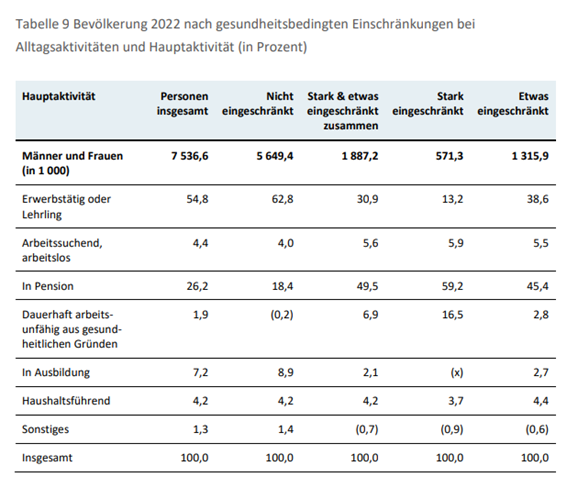
\includegraphics[scale=1]{pics/Statistik-Hauptaktivitaet.png}
    \caption{Statistik Hauptaktivitaet}
    \label{fig:statistik-2}
\end{figure}

(Quelle1, Quelle2)

\section{Interviews}
Im Rahmen eines Projekts bestand die Möglichkeit, einige Menschen kennenzulernen und 
mit diese Interviews über ihre Erfahrungen im Rollstuhl zu führen. Die Untersuchung zeigt, dass 
die zu bewältigende physische Herausforderung von emotionaler Stärke, dem Umgang mit der Umwelt 
sowie einem persönlichen Lebenswillen begleitet wurde, die sich auf unterschiedliche Weise äußerten. 
Die Gründe für die Pflegebedürftigkeit der Testpersonen waren heterogen. So waren die Betroffenen 
entweder dauerhaft oder vorübergehend auf einen Rollstuhl angewiesen. Ihre Geschichten demonstrieren 
die Diversität des Lebens mit einer Mobilitätseinschränkung und die Implikationen, die sich aus der 
Notwendigkeit ergeben, plötzlich oder von Geburt an auf Hilfe oder Hilfsmittel angewiesen 
zu sein.

\subsection{Zusammenfassung Interview 1}
Anna, 18 Jahre alt, erlitt vor vier Jahren einen schweren Unfall, in dessen Folge sie eine 
körperliche Beeinträchtigung erlitt, die für eine kurze Phase der Pflegebedürftigkeit in 
einem Rollstuhl erforderlich machte. Diese Wandelung vollzog sich in einem zeitlichen begrenzten, 
abrupten Ausmaß.

Nach dem Unfall wurde sie für die Dauer von einer Woche in ein Krankhaus gebracht. Sie sah sich 
mit der Herausforderung konfrontiert, sämtliche Alltagsaktivitäten neu zu erlenen. Hierzu zählten 
die eigenständige An- und Auskleidung sowie die Nutzung von Hilfsmitteln zur Körperpflege und die 
selbstständige Bedienung des Rollstuhls. Zunächst überwog eine ausgeprägte Verzweiflung. 
Allmählich manifestierte sich eine Veränderung. Es gelang ihr, sowohl eine physische als auch 
eine psychische Regeneration zu erfahren. Dennoch gestaltete sich der Übergang zurück in den 
Alltag als eine Abfolge kleiner, unerwarteter Schwierigkeiten. 

Nach dem Bruch ihrer Hüfte war Anna für die Dauer einer Woche auf einen Rollstuhl angewiesen für
eine kurze Zeit, jedoch stellte sie für sie eine völlig neue Erfahrung dar. Es wurde eine 
deutliche Verschlechterung der täglichen Routinen beobachtet, die sich in einfachen 
Verrichtungen wie dem Aufstehen am Morgen, dem Anziehen oder dem Duschen äußerte. Es oblag 
ihr, eine Vielzahl alltäglicher Abläufe neu zu erlernen oder dieses unter Zuhilfenahme von 
Hilfsmitteln zu bewältigen.

Der Schulbesuch stellte eine besondere Herausforderung dar. Das Gebäude entsprach nicht den 
Anforderungen der Barrierefreiheit, da es über keinen Aufzug verfügte, obwohl sich zahlreiche 
Unterrichtsräume in den oberen Stockwerken befanden. Die Bewältigung von Treppen stellt ein
Hindernis dar, die durch die physische und mentale Barriere der Überwindung charakterisiert ist. 
In viele Fällen war Improvisation unumgänglich. Die Schülerin wurde in andere 
Räumlichkeiten umgeleitet oder mit der Bearbeitung der Aufgaben zu Hause beauftragt. In der Folge 
verspürte sie eine Abkehr von der Klassengemeinschaft.

Die Zeit nach dem Unfall stellte sich zudem als eine physisch sowie psychisch belastenden Zeit 
heraus. Die plötzliche Notwendigkeit, auf die Unterstützung anderer angewiesen zu sein, 
beispielsweise beim Tragen der Schultasche, beim Öffnen von Türen oder beim Fortbewegen, wurde 
als ungewohnt und schmerzhaft empfunden. Die zuvor als selbstständig beschriebene Person sah 
sich plötzlich gezwungen, fortwährend um Hilfe zu ersuchen.

Besonders schwer wog dabei das Gefühl der Hilflosigkeit. Es 
ging einher mit der Angst, nie wieder vollständig zu genesen, und der Sorge, von anderen 
nur noch über die Verletzung definiert zu werden.

Obwohl sie den Rollstuhl nur temporär benötigte, führte diese Phase zu einer signifikanten 
Veränderung ihrer Perspektive auf zahlreiche Aspekte. Sie erlangte die Einsicht, dass sich das 
Leben mitunter rapide wandeln kann und dass es von großer Wichtigkeit ist, Geduld mit sich 
selbst zu bewahren.

\subsection{Zusammenfassung Interview 2}
Lukas, Alter 15, ist seit Mitte des Jahres 2024 auf einen Rollstuhl angewiesen, nachdem er 
infolge eines Unfalls für mehrere Monate immobil war. Die vorliegende Untersuchung widmet sich der
Thematik der Anpassung an eine neue körperliche Realität sowie den damit einhergehenden Veränderungen 
im alltäglichen Leben. Die Transition vom selbstständigen Gehen zur Nutzung eines Rollstuhls stellte 
eine einschneidende Erfahrung dar, die mit physischen und psychischen Herausforderungen einherging.

Der initiale Zustand des Alltags war durch eine signifikant ausgeprägte Fremdheit gekennzeichnet. 
Tätigkeiten, die zuvor als selbstverständlich erachtet wurden, wie das Überwinden von Stufen oder 
das selbstständige Bewegen über unebene Flächen, erforderten plötzlich fremde Hilfe. Die Abhängigkeit 
von anderen Personen wurde insbesondere in Bezug auf das Überwinden von Barrieren oder das Erreichen 
höhergelegener Orte als belastend empfunden. Im Zeitverlauf manifestierte sich eine zunehmende Routine. 
Lukas beschreibt, dass er sich in kurzer Zeit mit der Funktionsweise des Rollstuhls vertraut machte und 
die anfängliche Unsicherheit allmählich einer gewissen Selbstverständlichkeit wich.

Nichtsdestotrotz stellte die Mobilität eine Herausforderung dar. Er betont, dass Situationen ohne 
helfende Personen oft mit Anstrengung und Frustration verbunden waren. Wurde er von jemand anderem 
geschoben, so empfand er dies als ungewohnt und teilweise beunruhigend, da sich der Rollstuhl in
diesen Momenten instabiler und schneller anfühlte. Das Empfinden der Fremdbestimmung konstituierte 
eine mentale Hürde, die über die rein körperliche Einschränkung hinausging.

Besonders problematisch gestaltete sich die Situation im öffentlichen Verkehr. Obwohl Lukas in der 
Regel von einer Begleitperson unterstützt wurde, wiesen alltägliche Wege, etwa das Einsteigen in
Bus oder Zug, ein potenzielles Gefahrenpotential auf. Bereits geringfügige Unebenheiten, wie der 
Übergang von der Straße auf den Gehsteig, können als problematisch erachtet werden. Glücklicherweise 
blieb er von Stürzen verschont, war sich jedoch der ständigen Möglichkeit bewusst, dass solche 
Situationen leicht außer Kontrolle geraten können. Es liegen keine Erfahrungen mit elektrischen oder 
sportlichen Spezialrollstühlen vor. 

Die schulische Umgebung wurde von Lukas als barrierefrei beschrieben. Im Vergleich zu seiner früheren 
Schule, in der große Teile des Gebäudes nicht zugänglich waren, konnte er in seiner aktuellen 
Einrichtung fast alle Räume erreichen. Lediglich in Einzelfällen wurden Hindernisse festgestellt, 
die den Zugang erschwerten.

Seit Anfang 2025 ist Lukas wieder in der Lage, ohne Rollstuhl zu gehen. Die Phase der eingeschränkten
Mobilität hinterließ dennoch einen nachhaltigen Eindruck. Dies resultierte in einer vertieften 
Auseinandersetzung mit Themen wie Selbstständigkeit, Barrierefreiheit und gesellschaftlicher Inklusion. 
Obwohl er bislang keine Reisen ins Ausland unternommen hat, gab er an, dass er einen Aufenthalt in Wien 
absolviert hat. Dort habe er kaum Unterschiede zur Barrierefreiheit in Linz wahrgenommen.

Er äußert sich kritisch über den öffentlichen Verkehr. Insbesondere für Menschen, die vollständig auf 
den Rollstuhl angewiesen sind, ist der Einstieg in Züge oder Busse ohne fremde Hilfe nahezu unmöglich. 
In diesem Bereich wird ein erheblicher Bedarf an Verbesserungen identifiziert. Taxis und private Autos 
werden hingegen als die verlässlichsten und komfortabelsten Fortbewegungsmittel bezeichnet.

Zusammenfassend lässt sich festhalten, dass Lukas Erfahrung im Rollstuhl eine signifikante Veränderung 
seines Blicks auf den Alltag bewirkt hat. Es wurde ersichtlich, dass die physischen Grenzen urbaner 
Mobilität nicht die einzigen Faktoren sind, die in Bezug auf städtische Mobilität zu berücksichtigen 
sind. Darüber hinaus wurden auch die emotionalen Aspekte von Abhängigkeit, Unsicherheit und Anpassung 
evident. Trotz der temporären Natur dieser Einschränkung bleibt diese Zeit für ihn prägend, als Phase 
der Erkenntnis, wie fragil Selbstständigkeit sein kann und wie wesentlich Empathie und Barrierefreiheit 
im gesellschaftlichen Zusammenleben sind.


\subsection{Zusammenfassung Interview 3}
Tom, 32 Jahre alt, ist seitdem er geboren ist infolge einer körperlichen Beeinträchtigung, die eine 
dauerhafte Rollstuhlabhängigkeit bedingt, behindert. Sein Alltag ist geprägt von einer Kombination aus 
Routine, Anpassung und der permanenten Auseinandersetzung mit einer Umwelt, die nicht immer barrierefrei 
gestaltet ist. Die vorliegende Darstellung befasst sich mit den physischen und psychischen 
Herausforderungen, die das Leben im Rollstuhl mit sich bringt, sowie mit den gesellschaftlichen und 
infrastrukturellen Bedingungen, die seinen Alltag maßgeblich beeinflussen.

Das Fortbewegen auf unebenem Untergrund, etwa auf Kopfsteinpflaster oder auf schmalen, uneben Wegen, 
stellt für Tom eine erhebliche Herausforderung dar. Das Befahren solcher Flächen erfordert ein hohes Maß 
an Konzentration und Kraft. Er beschreibt das subjektive Empfinden als mühsam und unangenehm, da jede 
Bewegung abgebremst und erschüttert wird. In vielen Fällen ist eine nur sehr langsame Progredienz zu 
beobachten. Zudem besteht eine konstante Angst, das Gleichgewicht zu verlieren oder in einer Vertiefung 
des Geländes stecken zu bleiben. In solchen Momenten ist er gezwungen, seine Aufmerksamkeit vollständig 
auf die Bewegung zu richten, wodurch der eigentliche Spaziergang oder Ausflug an Leichtigkeit einbüßt.

Stufen, Bordsteinkanten und größere Höhenunterschiede stellen dabei die größten Herausforderungen dar. 
Während geringe Schwellen mit einer gewissen Dynamik überwunden werden können, stellen Treppen oder 
Bodenlücken eine unüberwindbare Barriere dar. In solchen Fällen ist Tom auf Unterstützung angewiesen, 
die zumeist durch Familienmitglieder oder Freunde erfolgt, die ihn begleiten. Die Analyse der vorliegenden 
Daten ergibt, dass Alleinreisen nur selten praktiziert werden können. Tom lebt mit seiner Familie, die 
ihn in den meisten Situationen unterstützt. Dennoch empfindet er es als belastend, nicht immer autonome 
Handlungsfähigkeit zu haben. Das Ersuchen um Unterstützung wird von ihm mit einem Gefühl der Abhängigkeit 
assoziiert, welches er nur schwer akzeptieren kann.

Tom misst der Gestaltung öffentlicher Räume eine besondere Bedeutung bei. Er betont, dass Rampen, 
barrierefreie Übergänge und glatte Wege die Lebensqualität von Rollstuhlnutzern erheblich steigern 
können. Als besonders positiv hebt er seine Erfahrungen an einem Strand hervor, an dem spezielle Wege 
bis hin zum Meer angelegt waren. Diese Fähigkeit ermöglichte es den Menschen, sich selbständig 
fortzubewegen und das Meer aus eigener Kraft zu erreichen. Dies vermittelte ihnen ein Gefühl von 
Freiheit und Selbstbestimmung.

Darüber hinaus verweist Tom auf die mangelnde Infrastruktur für Rollstuhlfahrer, etwa fehlende 
Parkplätze, zu enge Wege oder unzureichend angepasste Hotelzimmer. Insbesondere das Reisen stellt 
für ihn und seine Familie eine finanzielle und organisatorische Herausforderung dar. Hotels, die 
über rollstuhlgerechte Badezimmer und barrierefreie Zugänge verfügen, sind häufig mit höheren Kosten 
verbunden und in vielen Regionen nur begrenzt verfügbar.

Tom beobachtet zudem kulturelle Unterschiede im Umgang mit Menschen mit Behinderung. In einigen 
Kulturkreisen werden freundliche und hilfsbereite Absichten zwar positiv bewertet, jedoch zeigt Tom 
eine gewisse Skepsis gegenüber dieser, als übertrieben empfundenen Verhaltensweisen, die er mit Mitleid 
verbindet. Er bevorzugt einen natürlichen und respektvollen Umgang, der seine Beeinträchtigung nicht als 
ausschließlich bestimmenden Faktor betrachtet.

Mit zunehmendem Alter bemerkt auch seine Mutter, die ihn oft schiebt, dass die körperliche Belastung zunimmt. 
Das gemeinsame Unterwegssein wird zunehmend als belastend empfunden, sowohl von der Frau als auch von 
Tom empfunden. Dies veranschaulicht, dass Barrierefreiheit nicht nur den Betroffenen selbst, sondern auch 
deren Angehörigen zugutekommt.

Des Weiteren beschreibt Tom das unangenehme Gefühl, welches sich einstellt, wenn er, etwa während des 
Umsteigens aus dem Rollstuhl, von anderen beobachtet wird. In diesen Momenten verspürt er ein Gefühl 
der Exposition, Verletzlichkeit und Bewertung. Die Familie des Betroffenen zeigt eine hohe Aufmerksamkeit 
für die Wahl von Orten, die über Rampen verfügen, um das Eintreten solcher Situationen zu vermeiden.

Es lässt sich festhalten, dass der Alltag des Probanden von einem stetigen Wechsel zwischen 
Selbstständigkeit und Abhängigkeit geprägt ist. Seine Erfahrungen zeigen, dass die Gestaltung 
öffentlicher Räume, Straßen und Gebäude einen entscheidenden Einfluss darauf hat, in welchem Maß 
Menschen mit Mobilitätseinschränkungen am gesellschaftlichen Leben teilhaben können. Trotz zahlreicher 
Herausforderungen zeigt Tom eine bemerkenswerte Gelassenheit. Er erkennt in jeder barrierefreien Rampe, 
in jedem angepassten Raum einen Aspekt des gesellschaftlichen Fortschritts und ein Indiz dafür, dass 
Inklusion nicht nur ein theoretisches Ideal, sondern eine alltägliche Notwendigkeit ist.

(Quelle 3, 4, 5)